\documentclass[11pt]{article}
\usepackage[margin=1in]{geometry}
\usepackage{hyperref}
\usepackage{amsmath}
\usepackage{amssymb}
\usepackage{graphicx}
\usepackage{needspace}
\title{Finite-memory projection corrections as a diagnostic gate for cosmological consistency tests}
\author{Jozsef Olcsak}
\date{2026-05-19}
\begin{document}
\maketitle



\Needspace{10\baselineskip}
\subsection*{Abstract}

We introduce a bounded finite-memory projection operator for diagnostic
cosmological consistency tests. The operator is formulated as an effective
projection response over normalized depth, $W(x)=1+\rho x^3$, with a passive
memory-budget bound $\rho \leq 4$. The construction is not presented as a complete
cosmological model or a direct measurement claim. It is instead a disciplined
diagnostic module for comparing projected response shapes against
backreaction-aware distance consistency reconstructions. In a BAO-only
diagnostic reconstruction, the locked K2 window overlaps the full target
envelope. In an SN+BAO source-split stress test, strict median-sign matching
exhibits a localized tension; a reconstruction-aware sign-stability gate
keeps this tension classified as non-violating without widening the K2 window.
The result motivates a future full-likelihood comparison while preserving
explicit claim boundaries.

\Needspace{10\baselineskip}
\subsection*{1. Introduction}

Modern cosmological consistency tests increasingly distinguish background
expansion, light-propagation effects, curvature consistency, and cosmic
backreaction. A residual relative to a homogeneous FLRW reference model is
therefore not automatically evidence for new physics: it may arise from optical
sampling, reconstruction convention, averaging, or the choice of observable
combination.

Heinesen and Clifton recently emphasized that broad classes of cosmological
models can be separated by how they violate FLRW curvature-consistency tests
[1].
They isolate two especially relevant routes: deviations in optical properties
and deviations in large-scale expansion. This is naturally adjacent to the
older Dyer-Roeder optical-distance tradition, where light propagation through
clumpy matter distributions is treated separately from the homogeneous
background distance law [3,4]. Koksbang then applied this kind of
observable logic to constrain cosmic backreaction over an extended redshift
range, finding consistency with vanishing backreaction at one standard
deviation while also emphasizing that significant backreaction is not yet ruled
out [2]. These papers are useful here because they make the main methodological
lesson sharp: a projected cosmological residual must be tested against optical,
geometrical, and reconstruction degeneracies before it is interpreted.

This note develops a deliberately narrow finite-memory projection diagnostic
that can be placed alongside such tests. The objective is not to validate a full
physical model. Instead, we ask whether a predeclared, bounded
projection-memory operator can define a reproducible diagnostic window and
survive basic source-split stress tests.

The contribution is therefore threefold. First, we define a finite-memory
operator whose amplitude is bounded before comparison with reconstructed
diagnostics. Second, we give an explicit shape-selection rule that fixes the
cubic kernel from a small power-kernel family. Third, we state a sign-stability
policy for interpreting reconstructed diagnostic points whose median sign is
method-sensitive.

\Needspace{10\baselineskip}
\subsection*{2. Relation To Existing Diagnostic Ideas}

The present construction is closest in spirit to a consistency diagnostic, not
to a replacement background cosmology. In a standard FLRW interpretation,
distances, expansion rates, and curvature relations are locked together by the
assumed homogeneous geometry. A violation of one of these relations can point
to several different mechanisms: altered large-scale expansion, altered light
propagation, averaging effects, or reconstruction artifacts. This is why the
same residual pattern can be read very differently depending on whether one is
testing optical propagation, backreaction, or modified dynamics.

The finite-memory operator introduced here is designed to sit at this
interface. It does not start by changing the background Friedmann equations.
Instead, it asks whether a projected diagnostic response can carry a bounded
memory of accumulated depth. This makes it naturally comparable to
Dyer-Roeder-type optical reasoning, where light propagation through clumpy
matter is separated from the homogeneous reference law, and to modern
backreaction tests, where averaged expansion and observed distance relations
need not encode the same effective geometry.

The important difference is that the operator below is not an additional
free-form fitting function. Its amplitude and shape are constrained before the
diagnostic comparison. This is the main methodological point: the operator is
allowed to be phenomenological, but it is not allowed to become arbitrarily
elastic after seeing the reconstructed envelope.

For this reason, the most important object in the paper is not the specific
cubic formula by itself. The stronger contribution is the combination of a
bounded response window, a predeclared admissibility rule, and a
reconstruction-stability-aware interpretation policy.

\Needspace{10\baselineskip}
\subsection*{3. Effective Diagnostic Module}

Only the effective module needed for this note is used. We assume that an
observed consistency residual can be represented as a projected response over a
normalized depth coordinate,

\[
0 \leq x \leq 1 .
\]

The variable x should be read operationally: it orders the accumulated
projected response along the diagnostic light-path/reconstruction depth. In the
point-level diagnostic table below, the public packet uses the frozen
operational mapping

\[
x = z/z_{\max}
\]

over the tested SN+BAO redshift grid. This is a redshift-ordered diagnostic
coordinate, not a final physical identification of x with redshift and not a
new cosmological observable.

The finite-memory correction is a multiplicative response operator acting on a
baseline projected shape:

\[
K_2(x) = W(x)K_1(x).
\]

This note studies the locked K2 form

\[
W(x) = 1 + \rho x^3 .
\]

The form is intentionally simple. Its purpose is to test whether a bounded,
delayed, monotone memory response can be made reproducible before comparison
with diagnostic envelopes.

\begin{figure}[htbp]
\centering
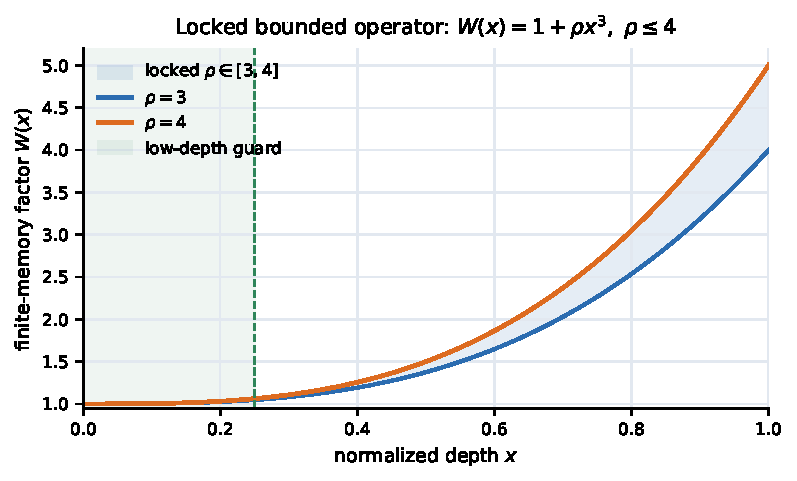
\includegraphics[width=0.95\textwidth]{figures/fig1_locked_operator.pdf}
\caption{Locked finite-memory operator. The shaded band is the predeclared $\rho\in[3,4]$ window inside the passive bound $\rho\leq4$; the low-depth guard shows why the response remains weak near the origin.}
\end{figure}

\Needspace{16\baselineskip}
\subsubsection*{Robustness And Coordinate Dependence}

The present note is coordinate-explicit. Its numerical tables use

\[
x = z/z_{\max}
\]

as the current frozen operational diagnostic mapping. This choice is useful
because it is simple, reproducible, and tied directly to the public redshift
grid. It is not claimed to be a coordinate-invariant or physically final
description of cosmological depth.

Two natural robustness mappings are left for the next stage:

\[
x = \chi(z)/\chi(z_{\max}),
\]

where $\chi$ is a comoving-distance coordinate under a frozen reference
cosmology, and an optical-depth-like coordinate in which the depth variable is
weighted by foreground or visibility information. A likelihood-native mapping,
using the reconstruction grid or likelihood coordinate directly, is the Phase II
target. Until such mappings are implemented, the method note should be read as
a coordinate-explicit diagnostic proposal only.

\Needspace{16\baselineskip}
\subsubsection*{K1 Baseline Provenance}

The baseline shape $K_1(x)$ is a frozen diagnostic baseline imported from the
distilled reconstruction packet. It is not fitted in this note. The comparison
is organized around whether the locked multiplicative memory factor can keep
the projected K2 response inside the reconstructed diagnostic envelope under
the predeclared amplitude and shape rules.

The present manuscript therefore tests the finite-memory multiplier on top of a
fixed diagnostic baseline. It does not establish that $K_1(x)$ is unique,
physically final, or likelihood-preferred.

Several assumptions are therefore intentionally modest:

\begin{itemize}
\item the coordinate $x$ is a diagnostic ordering variable, not a new directly measured cosmological coordinate;
\item the operator $W(x)$ is an effective response, not a complete field equation;
\item the reconstructed envelopes are treated as diagnostic targets, not as final likelihood surfaces;
\item the public module does not require the reader to accept any broader background theory.
\end{itemize}

These restrictions make the paper weaker than a full theory paper, but stronger
as a falsifiable method note. A reader can reject or test the effective module
without needing to adjudicate any larger research program.

\Needspace{10\baselineskip}
\subsection*{4. Passive Memory Bound}

The passive memory-budget condition requires the accumulated tail response not
to exceed the unit local response budget. For the cubic operator,

\[
E_{\mathrm{tail}} = \int_0^1 \rho x^3\,dx = \frac{\rho}{4}.
\]

The unit baseline budget is

\[
E_0 = \int_0^1 1\,dx = 1.
\]

Passivity requires

\[
E_{\mathrm{tail}} \leq E_0,\qquad
\frac{\rho}{4} \leq 1,\qquad
\rho \leq 4 .
\]

This is the key discipline of the construction: the memory depth is bounded
before the diagnostic comparison. The bound is not chosen by looking for the
best residual fit.

The word "passive" is used in this limited sense only. It means that the memory
tail does not carry more integrated response budget than the local baseline
term over the normalized interval. It does not mean that the underlying
cosmology is static, nor that no physical energy exchange is possible in a
deeper model. For this paper, passivity is simply a guard against an
uncontrolled late-depth amplification.

This bound also gives an immediate falsification handle. If a diagnostic
comparison requires $\rho > 4$ in order to remain compatible with the target
envelope, the locked passive operator is not supported in its present form. The
model is not then rescued by expanding the allowed amplitude range.

\Needspace{10\baselineskip}
\subsection*{5. Kernel-Shape Selection}

The cubic kernel is selected from the power-kernel family

\[
W_p(x) = 1 + \rho x^p .
\]

For this family, the passive memory rule generalizes to

\[
\int_0^1 \rho x^p\,dx \leq \int_0^1 1\,dx,\qquad
\frac{\rho}{p+1} \leq 1,\qquad
\rho \leq p+1 .
\]

Two additional effective-operator rules select the usable shape:

\[
\Delta W_p(0.25) = (p+1)0.25^p \leq 0.10 ,
\]

\[
\int_{0.75}^{1} (p+1)x^p\,dx \leq 0.75 .
\]

The first rule rejects kernels that disturb the already locked low-depth
response too early. The second rejects kernels whose memory budget collapses
too sharply onto the last quarter of the path. In the present audit, p=1 and
p=2 are too visible at low depth, while p>=4 is too endpoint-concentrated.
The cubic p=3 case is the remaining admissible power-kernel representative.

The locked diagnostic window is therefore

\[
W(x) = 1 + \rho x^3,\qquad
\eta \in [0.25,0.50],\qquad
\rho \in [3.00,4.00].
\]

The two shape rules encode a compromise. A linear or quadratic memory term
becomes visible too early and risks contaminating the low-depth regime where
the baseline diagnostic response should remain dominant. Higher powers delay
the response more strongly, but at the cost of concentrating the correction too
close to the endpoint. The cubic term is therefore not claimed to be uniquely
fundamental; it is the lowest simple power that is late enough at low depth
while not being too endpoint-like.

This distinction matters for interpretation. The paper does not say that
cosmology "must" use a cubic memory law. It says that, inside this deliberately
small power-kernel audit, the cubic law is the locked representative that
survives the predeclared admissibility rules.

The numerical thresholds in these two rules should also be read conservatively.
They are method thresholds for the present diagnostic packet, not universal
constants. A later likelihood paper should report threshold-sensitivity runs
showing whether the cubic representative remains selected when the low-depth
visibility and endpoint-concentration cuts are varied within a reasonable
predeclared range.

The current threshold-sensitivity policy is summarized as follows:

\begin{figure}[htbp]
\centering
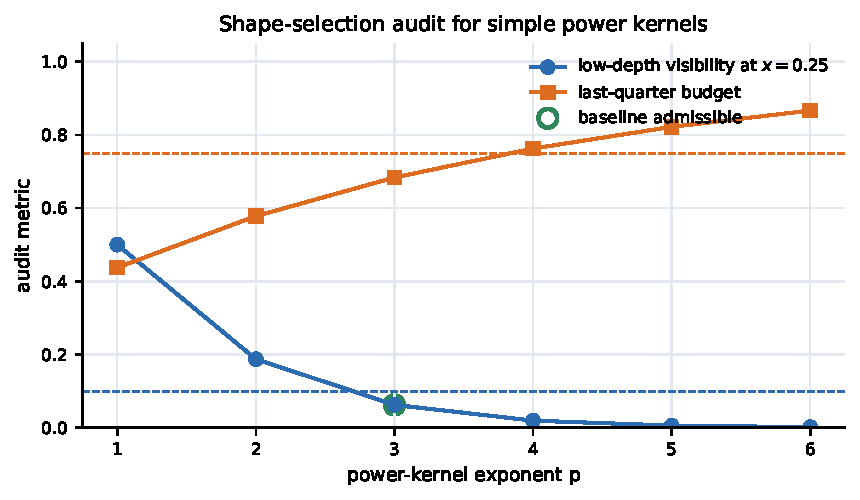
\includegraphics[width=0.95\textwidth]{figures/figA_threshold_sensitivity.pdf}
\caption{Power-kernel shape-selection audit. The cubic representative is selected by the current low-depth visibility and endpoint-budget thresholds; this is a methodological selection rule, not a fundamental-law claim.}
\end{figure}

\begin{center}
\begingroup
\scriptsize
\setlength{\tabcolsep}{3pt}
\renewcommand{\arraystretch}{1.15}
\resizebox{\textwidth}{!}{%
\begin{tabular}{lllll}
\hline
Threshold set & Low-depth limit & Endpoint budget & Admissible simple kernels & Interpretation \\
\hline
baseline & $\Delta W_p(0.25)\leq 0.10$ & endpoint $\leq 0.75$ & $p=3$ & cubic is the current audit-selected representative \\
relaxed low-depth & $\Delta W_p(0.25)\leq 0.15$ & endpoint $\leq 0.75$ & $p=2,3$ & more low-depth visibility broadens the set \\
strict low-depth & $\Delta W_p(0.25)\leq 0.075$ & endpoint $\leq 0.75$ & $p=3$ & cubic remains in this simple scan \\
relaxed endpoint & $\Delta W_p(0.25)\leq 0.10$ & endpoint $\leq 0.85$ & $p=3,4$ & endpoint relaxation admits a later kernel \\
strict endpoint & $\Delta W_p(0.25)\leq 0.10$ & endpoint $\leq 0.60$ & none & the simple power-kernel family can be emptied \\
\hline
\end{tabular}%
}
\endgroup
\end{center}

This means the cubic kernel is not a fundamental cosmological law. It is the
baseline representative selected by the current audit thresholds. Relaxing or
tightening those thresholds can broaden, shift, or empty the admissible simple
power-kernel set.

\Needspace{10\baselineskip}
\subsection*{6. Diagnostic Targets And Gate Policy}

The targets used here are reconstructed diagnostic envelopes rather than direct
published likelihoods. The comparison is therefore deliberately separated into
three levels:

\begin{verbatim}
sign-stable reconstructed point   -> exact sign gate
sign-unstable reconstructed point -> envelope / diagonal residual gate
controls and extrapolations       -> stress diagnostics only
\end{verbatim}

Operationally, let $y_i$ denote the reconstructed diagnostic median at the
tested point $i$, and let $[L_i,U_i]$ denote the corresponding reconstructed
diagnostic envelope. A locked prediction $\hat y_i$ is envelope-compatible
when

\[
L_i \leq \hat y_i \leq U_i .
\]

If a diagonal diagnostic width $\sigma_i$ is available, the normalized residual
gate is

\[
\left|\hat y_i-y_i\right|/\sigma_i \leq 1 .
\]

A reconstructed point is sign-stable only when the relevant method/degree
families agree on the sign of the diagnostic median. If the reconstruction
sign is method-sensitive, the median sign is not used as a hard falsifier.
Instead, the locked K2 prediction must remain inside the diagnostic envelope
and have a normalized residual not exceeding one standard diagnostic width.

This policy is not a substitute for a full likelihood. It is a triage rule that
prevents a method-sensitive reconstructed median from being overinterpreted.

This distinction is important for the SN+BAO stress test below. A strict
median-sign gate asks whether the prediction follows the sign of one
reconstructed median. The sign-stability gate asks a weaker but better-posed
question: whether the prediction violates a sign that is stable across
reconstruction choices. Only the second question is used as a paper-level
diagnostic violation/non-violation rule here.

\Needspace{10\baselineskip}
\subsection*{7. Source-Split Interpretation}

The BAO-only and SN+BAO diagnostics are not interchangeable. BAO-only
reconstructions are comparatively closer to a distance-scale consistency test,
while SN+BAO combinations mix distance ladder information and reconstruction
choices in a way that can sharpen or destabilize local features. A finite
memory operator should therefore not be judged only by whether it follows a
single reconstructed median. It should also be judged by whether a claimed
tension is robust across reconstruction families.

In the present packet, this is exactly where the localized SN+BAO warning
appears. The strict median-sign comparison identifies a point near z=1.1925
where the median sign is negative while the locked K2 response does not follow
that sign. The reconstruction audit, however, indicates that this sign is not
stable across the tested method/degree families. Lower-degree reconstructions
favor the opposite sign, while higher-degree reconstructions pull the median
negative.

The sign-stability policy is intended to prevent this point from being used in
either direction too aggressively. It should not be hidden, because it is a
real stress point for the diagnostic. It should also not be promoted to a hard
falsification, because the sign being tested is reconstruction-sensitive. The
paper-level statement is therefore deliberately asymmetric: the point remains a
warning, but not a locked diagnostic violation under the envelope and
normalized-residual gate.

\Needspace{10\baselineskip}
\subsection*{8. Results}

The minimal result summary is:

\begin{center}
\begingroup
\scriptsize
\setlength{\tabcolsep}{3pt}
\renewcommand{\arraystretch}{1.15}
\resizebox{\textwidth}{!}{%
\begin{tabular}{lll}
\hline
Diagnostic & Result & Interpretation \\
\hline
BAO-only window overlap & 1.0000000000 & Locked K2 overlaps the BAO-only diagnostic envelope at all tested points. \\
BAO-only best curve overlap & 1.0000000000 & The best locked K2 BAO-only curve remains inside the envelope. \\
SN+BAO sign-stable non-violation fraction & 1.0000000000 & All sign-stable SN+BAO points are non-violating under exact sign matching. \\
SN+BAO sign-unstable compatibility fraction & 1.0000000000 & All sign-unstable SN+BAO points remain envelope-compatible under diagonal residual handling. \\
\hline
\end{tabular}%
}
\endgroup
\end{center}

The strict SN+BAO median-sign test exhibits a localized tension near
z=1.1925. The diagnostic audit shows that this point is method-degree
sensitive: lower-degree reconstructions are positive, while higher-degree
reconstructions pull the median negative. The locked K2 prediction does not
follow the negative median sign at that point, but it remains inside the broad
diagnostic envelope with a small normalized residual. Under the sign-stability
gate, this is treated as an envelope-compatible warning rather than a hard
sign violation.

The current status is therefore:

\begin{verbatim}
BAO-only: diagnostic compatibility
SN+BAO strict median-sign: localized warning
SN+BAO sign-stability-aware gate: non-violating diagnostic status
claim level: theory-method diagnostic, not measurement validation
\end{verbatim}

\begin{figure}[htbp]
\centering
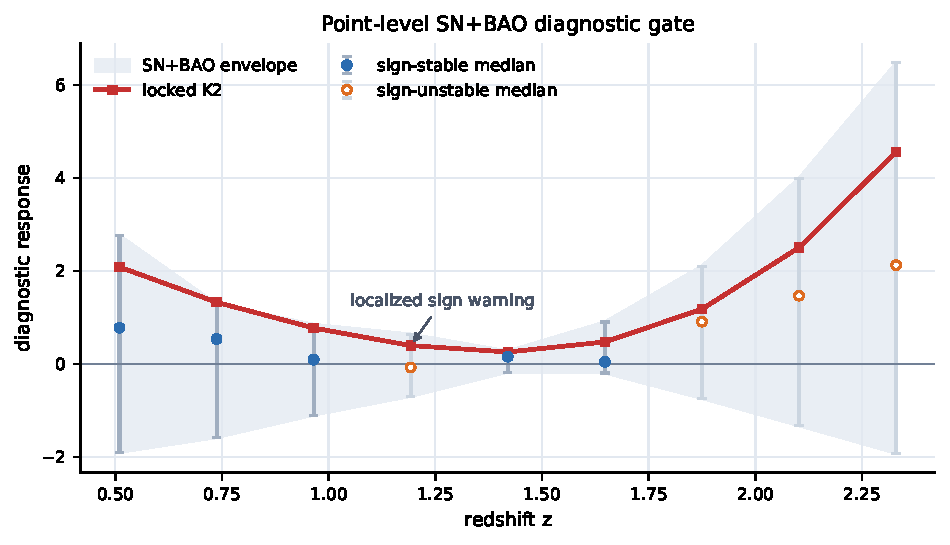
\includegraphics[width=0.95\textwidth]{figures/fig2_snbao_gate.pdf}
\caption{Point-level SN+BAO diagnostic gate. Filled points are sign-stable reconstructed medians, open points are sign-unstable medians, the grey band is the no-degree-4 robust envelope, and the red curve is the locked K2 prediction.}
\end{figure}

The point-level SN+BAO audit makes the gate policy more explicit. The source
for all rows is the no-degree-4 robust SN+BAO envelope, and the x column uses
the provisional mapping $x=z/z_{\max}$ over this grid.

\begin{center}
\begingroup
\scriptsize
\setlength{\tabcolsep}{3pt}
\renewcommand{\arraystretch}{1.15}
\resizebox{\textwidth}{!}{%
\begin{tabular}{lllllllll}
\hline
z & x & median & envelope & K2 & signs all/no4/d2 & stable? & residual/sigma & decision \\
\hline
0.5100 & 0.2189 & 0.7758 & [-1.9013, 2.7631] & 2.0829 & +/+/+ & yes & -0.0350 & NONVIOLATING\_SIGN\_STABLE \\
0.7375 & 0.3165 & 0.5350 & [-1.5846, 1.2890] & 1.3251 & +/+/+ & yes & -0.0565 & NONVIOLATING\_SIGN\_STABLE \\
0.9650 & 0.4142 & 0.0906 & [-1.1023, 0.8498] & 0.7717 & +/+/+ & yes & 0.1417 & NONVIOLATING\_SIGN\_STABLE \\
1.1925 & 0.5118 & -0.0762 & [-0.6967, 0.6401] & 0.3938 & -/-/+ & no & 0.1971 & COMPATIBLE\_SIGN\_UNSTABLE \\
1.4200 & 0.6094 & 0.1560 & [-0.1773, 0.2784] & 0.2554 & +/+/+ & yes & 0.0421 & NONVIOLATING\_SIGN\_STABLE \\
1.6475 & 0.7071 & 0.0445 & [-0.1959, 0.9010] & 0.4717 & +/+/+ & yes & 0.2289 & NONVIOLATING\_SIGN\_STABLE \\
1.8750 & 0.8047 & 0.9081 & [-0.7426, 2.1026] & 1.1769 & +/+/- & no & -0.1356 & COMPATIBLE\_SIGN\_UNSTABLE \\
2.1025 & 0.9024 & 1.4662 & [-1.3295, 3.9935] & 2.5013 & +/+/- & no & -0.0636 & COMPATIBLE\_SIGN\_UNSTABLE \\
2.3300 & 1.0000 & 2.1225 & [-1.9217, 6.4719] & 4.5595 & +/+/- & no & 0.0079 & COMPATIBLE\_SIGN\_UNSTABLE \\
\hline
\end{tabular}%
}
\endgroup
\end{center}

This table also makes the main weakness visible. The non-violation decisions are not
equivalent to a strong likelihood preference: several envelopes are broad, and
four of the nine SN+BAO points are sign-unstable. The table supports the narrow
claim that the locked K2 response does not violate the current diagnostic gate;
it does not support a direct measurement claim.

\Needspace{10\baselineskip}
\subsection*{9. Measurement Gate Preflight Status}

The measurement-gate scaffold is operational, but it remains a preflight
benchmark rather than a measurement-validation result. The purpose of the gate
is to keep the finite-memory projection hypothesis testable: the K2 operator is
locked before scoring, null comparators are registered in advance, and stronger
claims remain blocked until covariance-aware public benchmarks and calibrated
physical nulls are available.

\Needspace{16\baselineskip}
\subsubsection*{9.1 Preflight Status}

The current implementation shows five relevant facts. First, the BAO-only
diagnostic envelope remains compatible with the locked K2 window under the
current reconstruction-level packet. Second, the SN+BAO comparison contains a
localized sign-stability warning rather than a clean median-sign match. Third,
coordinate robustness is not automatic: an operator-only chi-normalized mapping
produces an envelope-tension warning, although bounded rho values within the
allowed rho <= 4 range can recover non-violating status in that diagnostic
stress test. Fourth, K1/no-memory remains competitive, and in some diagonal or
public-proxy scorecards it is stronger than fixed K2. Fifth, several
source-split and predeclared-protocol-guided preflight routes favor locked K2 over
local reproduction-family and backreaction-proxy controls, but these are not
likelihood-native measurement validations.

\Needspace{16\baselineskip}
\subsubsection*{9.2 Coordinate Robustness}

\begin{figure}[htbp]
\centering
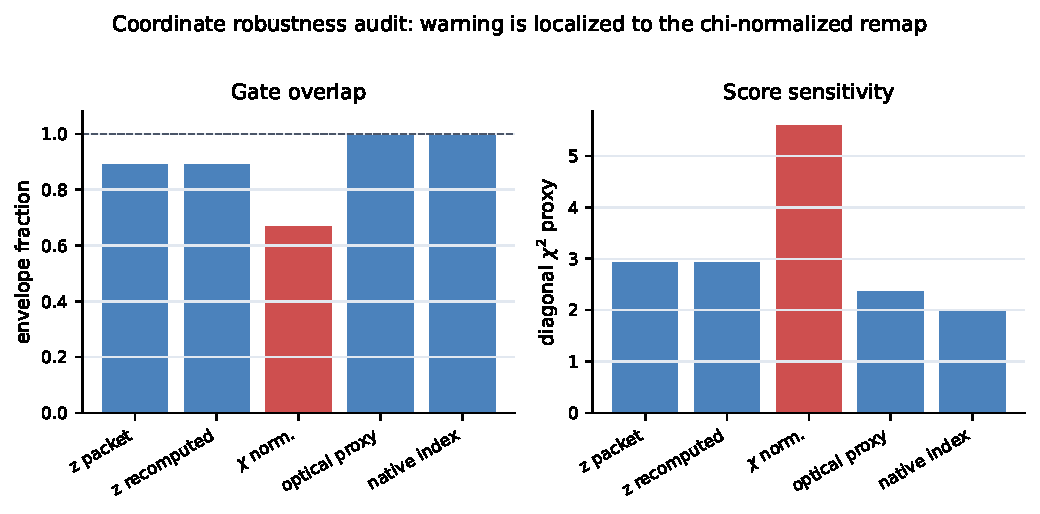
\includegraphics[width=0.95\textwidth]{figures/fig3_coordinate_robustness.pdf}
\caption{Coordinate robustness audit. Most mappings remain non-violating under the current gate, while the chi-normalized operator-only remap produces the localized coordinate warning that remains a Phase II target.}
\end{figure}

\Needspace{16\baselineskip}
\subsubsection*{9.3 Null Comparators}

\begin{figure}[htbp]
\centering
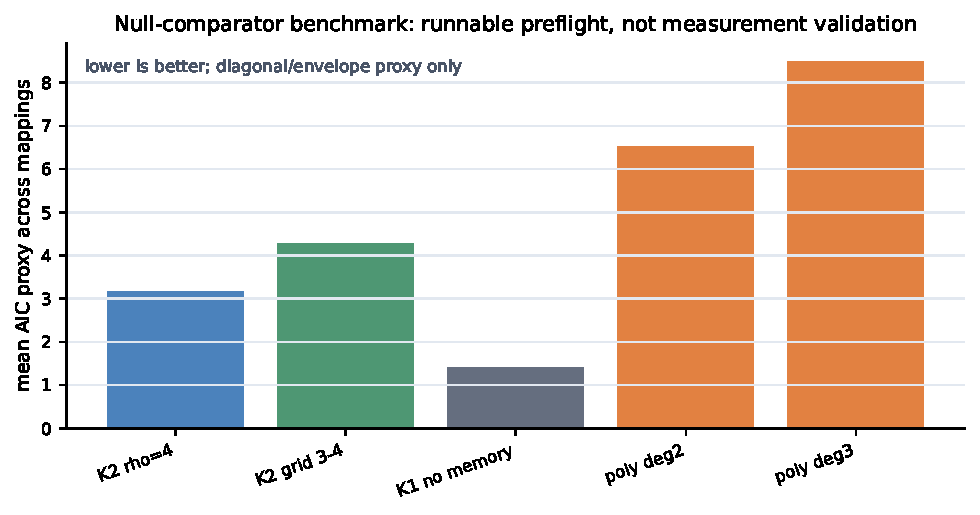
\includegraphics[width=0.95\textwidth]{figures/fig4_null_scorecard.pdf}
\caption{Null-comparator preflight scorecard. The chart reports proxy information-criterion scores across the current mappings; it is a benchmark diagnostic, not a measurement-validation result. These proxy scores are route-dependent and do not constitute likelihood-level model selection.}
\end{figure}

\Needspace{16\baselineskip}
\subsubsection*{9.4 Gate Closure Conditions}

Thus the measurement gate is useful precisely because it does not promote the
current result too far. The present package supports a disciplined diagnostic
claim: a bounded finite-memory operator can be locked, scored, compared with
nulls, and stress-tested reproducibly. It does not yet support a measurement
claim. The gate remains closed until the following objects are available:

\begin{itemize}
\item a likelihood-native K1/no-memory target;
\item a joint SN+BAO covariance or a preregistered shrinkage-covariance benchmark;
\item calibrated optical and backreaction physical-null comparators;
\item source-native or independently reproduced derivative/covariance exports for the backreaction route;
\item a frozen public benchmark in which no K2 kernel, rho bound, or K1 baseline is changed after scoring.
\end{itemize}

The detailed implementation log, including source-split export guards,
covariance registries, predeclared-protocol-guided reproduction families, and
backreaction preflight audits, is retained in the public repository as
docs/measurement\_gate\_audit\_log.md.

\Needspace{10\baselineskip}
\subsection*{10. Robustness And Falsification Criteria}

The current evidence is deliberately weaker than a full likelihood. For that
reason, it is useful to state what would make the finite-memory diagnostic fail
or become substantially less interesting.

The diagnostic would fail in its present form if:

\begin{itemize}
\item the BAO-only envelope overlap disappeared under the same locked K2 window;
\item sign-stable SN+BAO points required the opposite sign from the locked prediction;
\item compatibility required $\rho > 4$ or a different kernel power chosen after seeing the envelope;
\item the localized SN+BAO warning became sign-stable under a stronger reconstruction audit;
\item a full covariance likelihood rejected the whole locked window rather than merely shifting the best point inside it.
\end{itemize}

Conversely, the diagnostic would become more interesting if the same locked
window survived a covariance-aware likelihood test, if independent
reconstructions selected a similar late-depth response shape, or if
backreaction-aware and optical-propagation tests separated in a way naturally
tracked by the K2 window.

These criteria are included to keep the method honest. The finite-memory
operator is useful only if it remains constrained. If it must be repeatedly
relaxed to follow each new diagnostic reconstruction, it loses the main
advantage of being predeclared.

\Needspace{10\baselineskip}
\subsection*{11. Expected Significance}

The main significance of the construction is not that it establishes a new
cosmological model. Its value is methodological:

\begin{itemize}
\item it gives a compact finite-memory operator whose amplitude is bounded before comparison with data;
\item it interfaces naturally with FLRW consistency, optical-propagation, and backreaction tests;
\item it demonstrates a way to handle sign-unstable reconstructed diagnostics without silently overclaiming;
\item it provides a small public module that can be tested independently as a diagnostic proposal.
\end{itemize}

The near-term audience is likely narrow: researchers interested in
cosmological consistency tests, backreaction, light propagation, and
method-level modified-gravity phenomenology. The higher-impact route requires
a later full covariance or shrinkage-covariance likelihood comparison with
direct public likelihood products.

\Needspace{10\baselineskip}
\subsection*{12. Limitations}

This manuscript is a theory-method diagnostic note. It does not claim:

\begin{itemize}
\item a full covariance likelihood;
\item a direct measurement claim;
\item exclusion of cosmic backreaction;
\item a complete derivation of cosmology from an underlying action;
\item reconstruction of a full background theory.
\end{itemize}

The next stage is a paper-aligned likelihood comparison using covariance or
shrinkage-covariance products and direct published likelihood data where
available.

The most important limitation is that the public packet contains distilled
diagnostic summaries rather than the full reconstruction pipeline. This is
acceptable for a method note whose purpose is to define a bounded operator and
state claim boundaries, but it is not sufficient for an observational paper.
The current manuscript should therefore be read as a bridge from a compact
diagnostic construction to a public, testable effective module, while leaving
the stronger likelihood comparison for a later release.

\Needspace{10\baselineskip}
\subsection*{13. Phase II Roadmap}

The next technical step is to replace the diagonal/envelope diagnostic with a
likelihood-level comparison. At minimum, this requires public likelihood or
data products, a covariance or shrinkage-covariance prescription, and a frozen
mapping from the reconstructed observable to the finite-memory diagnostic
coordinate $x$.

A useful future workflow is:

\begin{verbatim}
freeze K2 window -> ingest public likelihood products -> build covariance-aware
diagnostic -> compare locked window -> report posterior support or rejection
\end{verbatim}

This future comparison should not widen the K2 window unless a new paper is
explicitly framed as a different model. The main value of the present note is
that it fixes a small target before the stronger test is performed.

The Phase II work package should therefore include:

\begin{itemize}
\item covariance-aware likelihood ingestion;
\item null comparators for no-memory, smooth-response, optical-propagation, and backreaction-only alternatives;
\item a public reconstruction benchmark;
\item coordinate-mapping robustness across redshift-normalized, comoving-distance, optical-depth-like, and likelihood-native coordinates;
\item direct comparison against BAO-only and SN+BAO reconstruction families;
\item a frozen benchmark challenge in which the K2 window is locked before testing.
\end{itemize}

\begin{figure}[htbp]
\centering
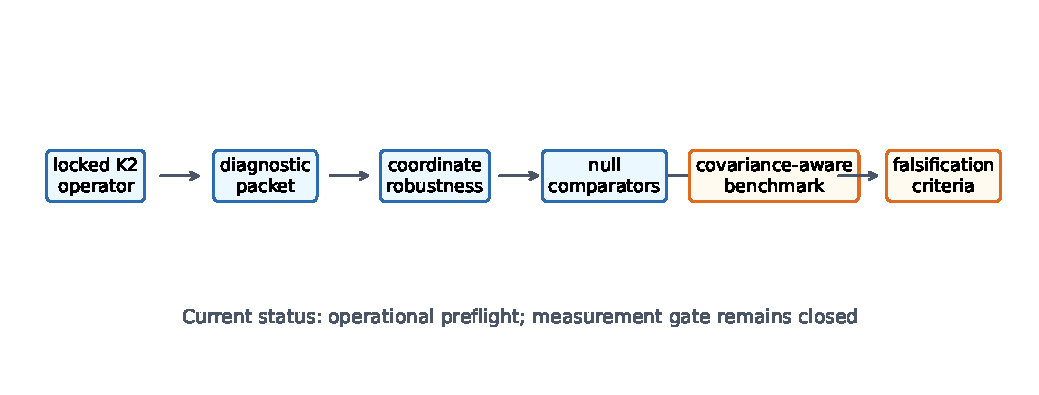
\includegraphics[width=0.95\textwidth]{figures/figB_measurement_gate_flow.pdf}
\caption{Measurement-gate preflight workflow. The current repository implements the left-hand preflight stages; the covariance-aware benchmark and falsification criteria remain the required route to stronger empirical claims.}
\end{figure}

\Needspace{10\baselineskip}
\subsection*{14. Conclusion}

We have defined a finite-memory projection correction as a bounded diagnostic
operator rather than as a complete cosmological model. The locked cubic form
$W(x)=1+\rho x^3$ follows from a passive memory budget and a simple
shape-selection audit over power kernels. With $\rho \leq 4$, the operator gives
a compact K2 diagnostic window that can be compared against reconstructed
cosmological consistency envelopes without fitting the memory depth after the
fact.

Within the distilled diagnostic packet used here, the locked K2 window is
compatible with the BAO-only envelope and remains non-violating under the
reconstruction-aware SN+BAO sign-stability gate. The strict SN+BAO median-sign
warning is retained as a limitation rather than hidden: it marks a
reconstruction-sensitive point that should be revisited with direct likelihood
products.

The result is therefore a release-candidate method-note claim, not an
measurement-validation claim. Its next meaningful test is a covariance-aware
likelihood comparison against public likelihood data and predeclared null
comparators.

\Needspace{10\baselineskip}
\subsection*{15. Data And Code Availability}

The public Paper 5 repository is hosted at
https://github.com/tau-core-research/finite-memory-cosmology-paper5. It
contains the manuscript source, rendered PDF, reproducibility scripts, derived
input packets, audit summaries, and the arXiv-style source archive.

The most important repository paths are:

\begin{itemize}
\item paper5\_submission\_source/: paper-facing draft, LaTeX facsimile, and PDF;
\item figures/: rendered manuscript figures in PDF and PNG form;
\item src/fmc/: scoring, covariance, coordinate, operator, and backreaction helper code;
\item scripts/: executable reproduction and audit scripts;
\item data/: derived public-input and local reproduction packets;
\item evidence/: compact CSV outputs used by the manuscript and audit gates;
\item docs/measurement\_gate\_audit\_log.md: detailed implementation/audit log moved out of the main paper;
\item frozen/: locked operator and configuration artifacts;
\item tests/: public reproducibility checks.
\end{itemize}

The key manuscript-facing outputs are:

\begin{itemize}
\item evidence/gate\_results\_current.csv;
\item evidence/finite\_memory\_preflight\_summary.csv;
\item evidence/registered\_protocol\_guided\_dominance\_summary.csv;
\item evidence/source\_native\_reproduction\_family\_dominance\_summary.csv;
\item finite\_memory\_projection\_corrections.pdf;
\item arxiv\_submission\_source.zip.
\end{itemize}

The current comparison should be treated as reconstruction-level diagnostic
preflight. Raw survey data and unpublished source-native derivative exports are not
redistributed. Source-native derivative/covariance exports remain a blocker for
measurement-validation language.

The current package can be regenerated with:

\begin{verbatim}
python3 -m pip install -r requirements.txt
PYTHONPATH=src python scripts/run_gate_current_packet.py
PYTHONPATH=src python scripts/build_finite_memory_preflight_packet.py
python studies/finite_memory_cosmology_paper5_v01/make_paper5_submission_source_v01.py
python -m pytest -q
\end{verbatim}

\Needspace{10\baselineskip}
\subsection*{References}

[1] A. Heinesen and T. Clifton, "Observational Tests for Distinguishing Classes
of Cosmological Models", arXiv:2604.07244, 2026.
https://arxiv.org/abs/2604.07244

[2] S. M. Koksbang, "First observational constraints on cosmic backreaction
over an extended redshift range", arXiv:2604.11249, 2026.
https://arxiv.org/abs/2604.11249

[3] C. C. Dyer and R. C. Roeder, "The Distance-Redshift Relation for Universes
with No Intergalactic Medium", The Astrophysical Journal 174, L115-L117,
1972.

[4] C. C. Dyer and R. C. Roeder, "Distance-Redshift Relations for Universes
with Some Intergalactic Medium", The Astrophysical Journal 180, L31-L34,
1973.

\end{document}
